%-*- coding: utf-8 -*-
\documentclass{beamer}

\usepackage[frenchb]{babel}
\usepackage[T1]{fontenc}
\usepackage[utf8]{inputenc}
\graphicspath{{images/}}

\usetheme{Warsaw}

\title{Projet Vitameal}
\subtitle{Restauration en milieu hospitalier}
\author{Nicolas Symphorien, Sonia Othmani, Jean-Félix Benitez}
\institute{CNAM}
\date{12/05/2017}

\logo{
\includegraphics[height=10mm]{ipst-cnam.png}}
\setbeamertemplate{background canvas}{
\includegraphics[width=\paperwidth,height=\paperheight]{fond_200.png}} % Width pour la largeur, height pour la hauteur de l'image

\begin{document}
\begin{frame}[plain]
  \titlepage
\end{frame}

\begin{frame}
  \frametitle{Sommaire}
  \tableofcontents
\end{frame}

\section{Définition du problème}
\begin{frame}[label=definitionDuProbleme]
\frametitle{Définition du problème}
L'élaboration de menus dans un hôpital pour la restauration des patients
est une tâche complexe, et doit tenir compte des différentes pathologies
rencontrées. Faute de moyens (temps et argent) seules quelques grandes
lignes de restauration sont retenues; alors qu'idéalement, chaque
patient devrait pourvoir avoir un repas adapté à sa pathologie.
\end{frame}

\subsection{Solution envisagée}
\begin{frame}[label=solutionEnvisagée]
\frametitle{Solution envisagée}
Le projet Vitameal a pour objectif de faire correspondre au mieux la planification des régimes et des
prescriptions diététiques aux repas réellement servis au patient. Il consiste en un outil interfaçant la
gestion de production, la prise de commande et le suivi nutritionnel des repas.
\end{frame}

\subsection{Périmètre}
\begin{frame}[label=perimetre]
\frametitle{Périmètre}
C'est un diététicien qui renseigne le profil diététique des patients,
sous les directives des médecins. C'est aussi un diététicien qui élabore
les menus des patients. L'outil élaborera donc
les menus par filtrage des produits correspondants aux profils
diététiques des patients. Pour des raisons de simplifications, nous nous limiterons dans ce projet aux seuls patients adolescents et adultes, à l'exclusion des personnes agées.
\end{frame}

\section{Analyse des exigences}
\begin{frame}[label=analyseDesExigences] %allowframebreaks
\frametitle{Analyse des exigences}
\begin{itemize}
  \item Partie prenantes
  \begin{itemize}
    \item Participantes~: les diététiciens, le service restauration
    \item Concernés~: les médecins, la direction (budget)
    \item Impactées~: les patients
  \end{itemize}
  \item Les besoins
  \begin{itemize}
    \item Les diététiciens renseignent les profils diététiques de chaque patient.
    \item Les diététiciens lance l'élaboration automatique des menus.
    \item Le service restauration commande les produits et ingrédients mis en œuvre dans les menus
    \item Le service restauration prépare les menus élaborés.
  \end{itemize}
  \item Les contraintes
  \begin{itemize}
    \item Les médecins doivent pouvoir vérifier / valider les profils diététiques des patients.
    \item La direction fixe un budget maximum par menu.
  \end{itemize}
\end{itemize}
\end{frame}

\subsection{Exigences}
\begin{frame}
 \frametitle{Exigences}
Chaque exigence est composée de 11 champs:
\begin{itemize}
\item \textbf{numéro:} Formé comme suit REQ\_12345
\item \textbf{Titre:} Titre ou description courte
\item \textbf{Corps:} Expression de l'exigence
\item \textbf{Type:} Utilisateur, Métier, Système, Contrainte
\item \textbf{Nature:} Fonctionnelle, Ergonomie, Robustesse, Performance, Sécurité
\item \textbf{Origine:} D'où vient une exigence ?
\item \textbf{Version:} ou niveau de maturité, Initiale, Intermédiaire, Finale
\item \textbf{Priorité:} MoSCoW, Must, Should, Could, Won't
\item \textbf{Validée:} L'exigences a-t-elle été validée ? (Oui / Non)
\item \textbf{Liens:} Liens
\item \textbf{Test:} Définition du test qui validera l'exigence.
\end{itemize}

\url{../../Exigences/Exigences.html}
\end{frame}

\subsection{Cas d'utilisations}
\begin{frame}
 \frametitle{Cas d'utilisations}
%-*- coding: utf-8 -*-
\subsubsection{Élaboration des menus}
\begin{figure}
  \centering
      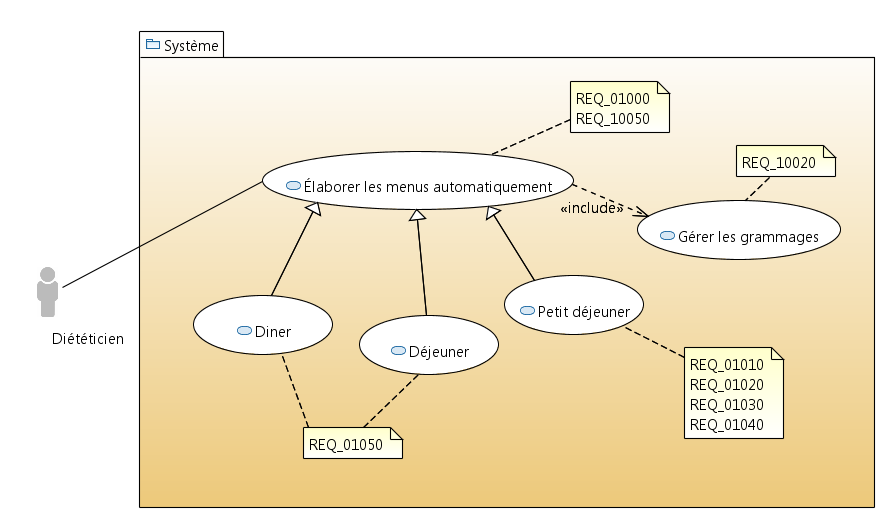
\includegraphics[width=1.00\textwidth]{../../CasDUtilisations/MenuGen/CasDUtilisation/MenuGen.png} %
\caption{Cas d'utilisation élaboration des menus}
\label{MenuGenCU}
\end{figure}

\begin{description}
\item[Nom:] Élaboration des menus (Figure \ref{MenuGenCU}).
\item[ID:] UC300
\item[Description:] Permet l'élaboration des menus.
\item[Auteur:] Jean-Félix BENITEZ.
\item[Date:] 15/06/2017
\item[Acteurs:] Diététiciens.
\item[Pré-Conditions:] Le diététicien s'est connecté au système.
\item[Scénario principal:] Figure \ref{MenuGenSeq}
  \begin{enumerate}
  \item Le diététicien sélectionne le groupe de patients pour lequel il veut générer les menus,
  \item \label{LanceElab}ensuite il lance l'élaboration des menus.
  \item L'élaboration automatique ce déroule en prenant en compte les grammages.
  \item Lorsque les menus sont élaborés, s'il estime l'élaboration correcte, il la valide.
  \item S'il estime l'élaboration incorrecte, il peut la rejeter, auquel cas il reviens à l'étape \ref{LanceElab}
  \item S'il estime l'élaboration incorrecte, il peut aussi la modifier manuellement.
  \end{enumerate}
\item[Scénario alternatif:] Aucun.
\item[Post-Conditions:] Les menus sont générés.
\end{description}

\begin{figure}
  \centering
      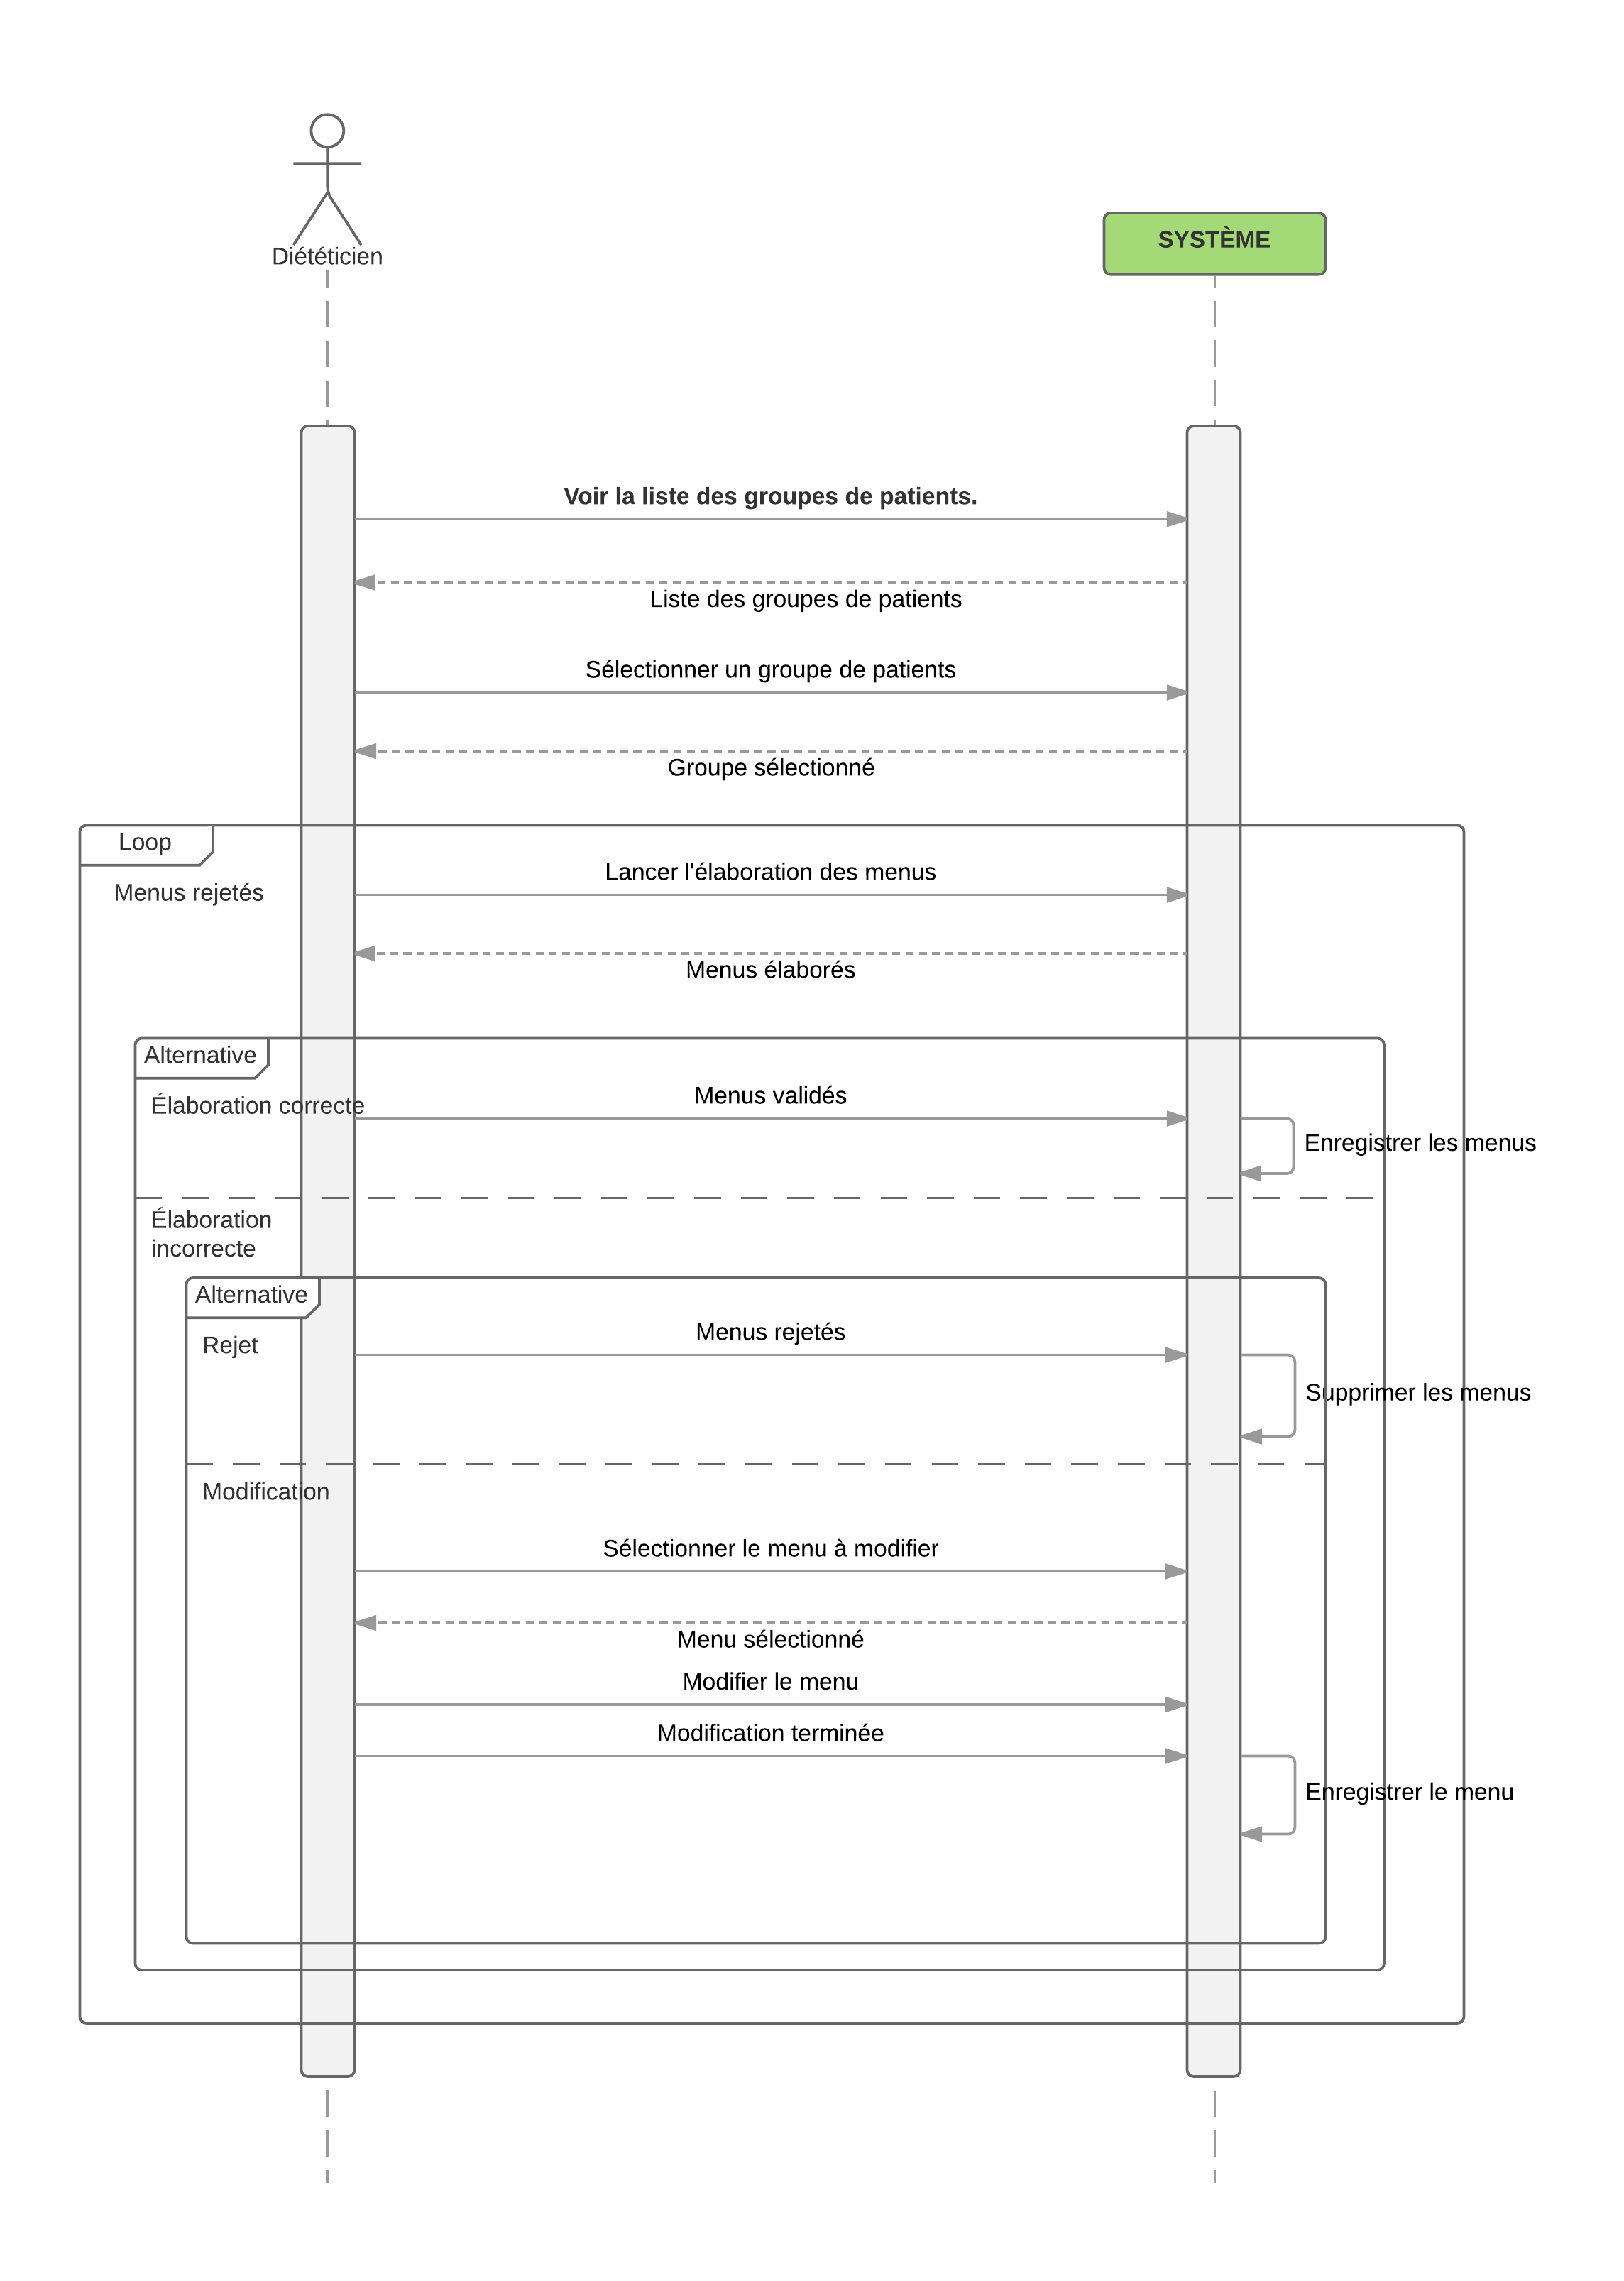
\includegraphics[width=1.00\textwidth]{../../CasDUtilisations/MenuGen/Sequence/ElaborationMenus.png} %
\caption{Séquence élaboration des menus}
\label{MenuGenSeq}
\end{figure}

\end{frame}

\section{Planning}
\begin{frame}[label=planning]
\frametitle{Planning}
\begin{figure}[H]
\textbf{G}antt
\label{Gantt}
  \centering
      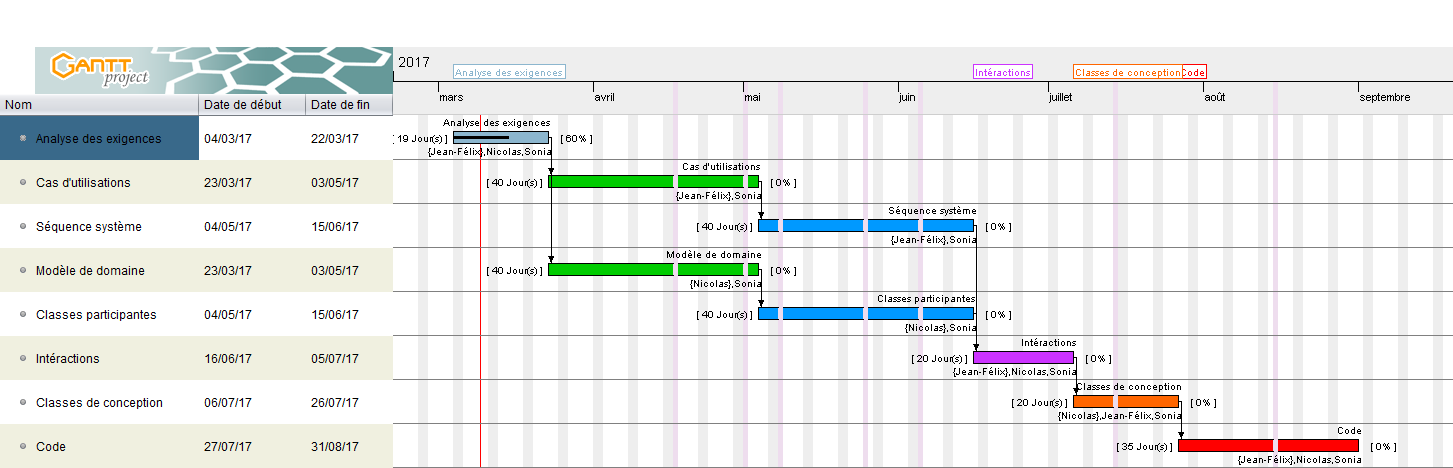
\includegraphics[width=0.95\textwidth]{Vitameal_gantt.png} %
%\caption{Gantt}
\end{figure}

\begin{figure}[H]
\textbf{P}rogram \textbf{E}valuation and \textbf{R}eview \textbf{T}echnique
\label{PERT}
  \centering
      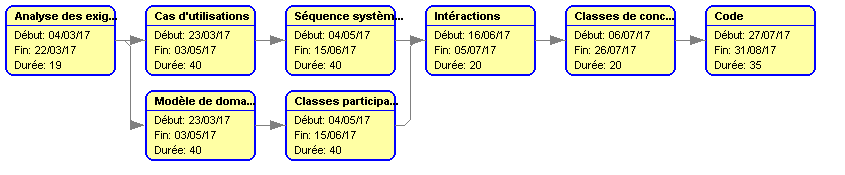
\includegraphics[width=0.95\textwidth]{Vitameal_pert.png} %
%\caption{PERT}
\end{figure}
\end{frame}

\section{Usine logicielle}
\begin{frame}[label=usineLogicielle]
\frametitle{Usine logicielle}
L'usine logicielle de Vitameal répond aux exigences suivantes :
\begin{itemize}
\item respecter les règles de qualités ;
\item avoir une documentation claire et intégrée au projet ;
\item gérer les erreurs et assurer leurs suivies ;
\item versionner le code source et la documentation ;
\item avoir un espace commun accessible à distance ;
\item gérer un espace de livraison générant des indicateurs de santé sur le projet ;
\item avoir un outil de conception UML couvrant la méthode minimal UML;
\item gérer la planification du projet.
\end{itemize}
\end{frame}

\subsection{Documentation}
\begin{frame}[label=documentation]
  \frametitle{Usine logicielle - Documentation}
  \begin{itemize}
  \item utilisation de la syntaxe \textbf{markdown};
  \item intégration à \textbf{GitHub};
  \item usage de \textbf{LaTex} pour les livrables
\end{itemize}
\end{frame}

\subsection{Poste de développement}
\begin{frame}[label=posteDeveloppement]
  \frametitle{Usine logicielle - Poste de Développement}
  \begin{itemize}
  \item \textbf{Eclipse} comme IDE pour écrire/éditer le code de l'application ;
  \item \textbf{Maven} comme constructeur du projet (gestion des dépendances, automatisation de la construction)
  \item \textbf{JUnit} pour écrire les tests unitaires de l'application et Coderturapour analyser la couverture du projet par ces tests ;
  \item \textbf{Git} pour versionnerles sources du projet ;
  \item \textbf{StarUML} pour modéliser selon le standard UML le projet ;
  \item \textbf{GanttProject} pour planifier le projet avec un diagramme de Gantt ;
  \item \textbf{TEXMaker} pour éditer les fichiers «.tex» avec un comportement proche des WYSIWYG (optionnel).
\end{itemize}  
\end{frame}

\subsection{Espace d'intégration continue}
\begin{frame}[label=integrationContinue]
  \frametitle{Usine logicielle - Espace d’intégration continue}
  \begin{itemize}
  \item \textbf{GitHub} comme gestionnaire à distance du repositorie \textbf{Git} principal, comme tracker de bug et comme affichage visuel des taches à faire ;
  \item \textbf{Jenkins} comme serveur d'intégration continue ;
  \item \textbf{SonarQube} comme analyseur de qualité du code.
  \end{itemize}
\end{frame}

\subsection{Schéma de fonctionnement}
\begin{frame}[label=schemaFonctionnement]
  \frametitle{Usine logicielle - Schéma de fonctionnement}
\begin{figure}[H]
\label{schema}
  \centering
      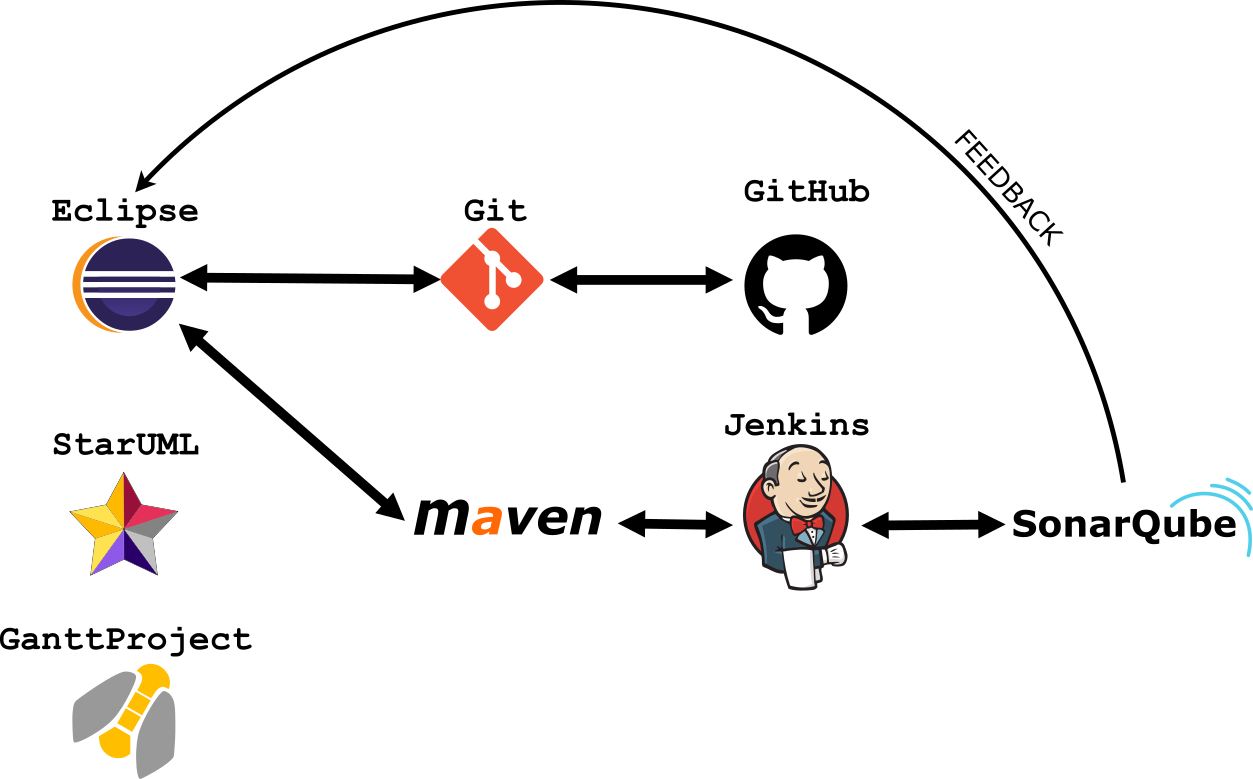
\includegraphics[width=1.0\textwidth]{usine_vitameal.png} %
%\caption{Schéma}
\end{figure}
\end{frame}

\end{document}
